\documentclass[a4paper]{article}

\usepackage{amsmath,amsthm,amssymb}
\usepackage{tikz}
\usetikzlibrary{arrows}
\usetikzlibrary{external}
\tikzexternalize[prefix=figures/]

\tikzset{
every node/.style={circle, draw, inner sep=2pt},
every label/.style={rectangle, draw=none}
}

\begin{document}

%%%%%%%%%%%%%%%%%%%%%%%%%%%%%%%%%%%%%%%%%%%%%%%%%%
\verb|randomwalk0|

\tikzsetnextfilename{randomwalk0}
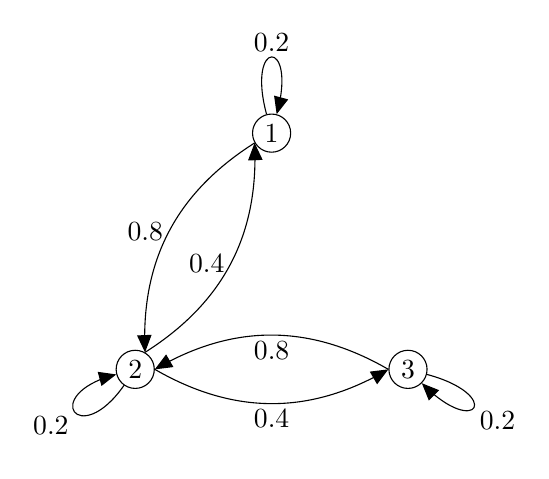
\begin{tikzpicture}[every loop/.style={min distance=10mm}]
\node (1) at (90:2) {$1$};
\node (2) at (210:2) {$2$};
\node (3) at (330:2) {$3$};

\draw[-triangle 45, bend right] (1.210) to node[midway, left, draw=none, rectangle]{$0.8$} (2.60);
\draw[-triangle 45, bend right] (2.0) to node[midway, below, draw=none, rectangle]{$0.4$} (3.180);
\draw[-triangle 45, bend right] (3.180) to node[midway, below, draw=none, rectangle]{$0.8$} (2.0);
\draw[-triangle 45, bend right] (2.60) to node[midway, left, draw=none, rectangle]{$0.4$} (1.210);

\draw[-triangle 45] (1) to[loop above] node[midway, draw=none, rectangle, above] {$0.2$} ();
\draw[-triangle 45] (2) to[out=235, in=195, loop] node[midway, draw=none, rectangle, anchor=30] {$0.2$} ();
\draw[-triangle 45] (3) to[out=345, in=315, loop] node[midway, draw=none, rectangle, anchor=150] {$0.2$} ();
\end{tikzpicture}


\end{document}


%%% compile by pdflatex --shell-escape filename.tex
%%% then run ./pdf2png.sh *.pdf in figures/
